\section{Schwingungen und Wellen}
\begin{auf}
    683
\end{auf}
Senkrecht unter dem Aufhängepunkt A eines mathematischen Pendels der Pendellänge $l_1=1.0m$ befindet sich ein Stift S, an den sich der Pendelfaden beim Zurückschwingen anlegt (Pendelhemmung). Das Pendel schwingt dann nach rechts mit der verkürzten Pendellänge $l_2$.
\begin{enumerate}
    \item[a] Wie groß ist der Abstand des Stiftes vom Aufhängepunkt, wenn die Schwingungsdauer für beide Halbschwingungen zusammen $T=1.5s$ beträgt?
    \item[b] Wie hoch schwingt die Pendelmasse nach rechts aus, wenn das Pendel um $\varphi_1=3.0^\circ$ nach links ausgelenkt und	dann losgelassen wird?
    \item[c] Wie groß ist der maximale Auslenkungswinkel $\varphi_2$ beim Ausschwingen nach rechts?
\end{enumerate}
\begin{figure}[h]
    \centering
    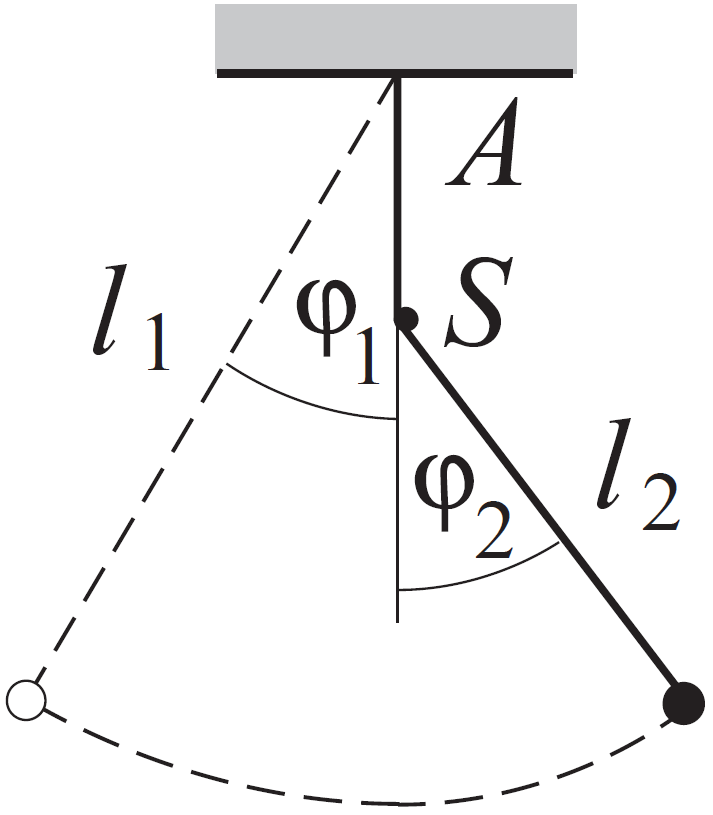
\includegraphics[height=5cm]{images/683_0.png}
    \caption{Versuchsaufbau Aufgabe 683}
\end{figure}